\section{Self-Suspending Tasks in Multiprocessor Synchronizations}
\label{sec:syn}

In this section, we consider multiprocessors the analysis of self-suspensions that arise on multiprocessors under \emph{partitioned fixed-priority (P-FP)} scheduling when tasks synchronize access to shared resources (\eg, shared I/O devices, communication buffers, or scheduler locks) with suspension-based locks (\eg, binary semaphores). Unfortunately, some of the misconceptions surrounding the analysis of self-suspensions on uniprocessors also spread to the analysis of partitioned multiprocessor real-time locking protocols. In particular, as we show with a counterexample, the analysis framework to account for the additional interference due to \emph{remote blocking} first introduced by \cite{lakshmanan-2009}, and reused in several other works~\cite{zeng-2011,bbb-2013,yang-2013,kim-2014,han-2014,carminati-2014,yang-2014},  is flawed. Finally, a straightforward solution for these problems is discussed. 

\subsection{Existing analysis strategies}
\label{sec:papers}

P-FP scheduling is a widespread choice in practice due to the wide support in industrial standards such as AUTOSAR, and in many RTOSs like VxWorks, RTEMS, ThreadX, \etc Under P-FP scheduling, each task has a fixed base priority and is statically assigned to a specific processor, and each processor is scheduled independently as a uniprocessor. 

Under partitioned scheduling, a resource accessed by tasks from different processors is called a \emph{global resource}, otherwise it is called a \emph{local resource}. When a job requests a global resource, it may incur \emph{remote blocking} if the global resource is held by a job on another processor. Also, a job may incur \emph{local blocking} if it is prevented from being scheduled by a resource-holding job of a lower-priority task on its local processor. 

Under suspension-based protocols, such as the \emph{multiprocessor priority ceiling protocol (MPCP)}~\cite{rajkumar-1990}, tasks that are denied to access shared resources are suspended. From the perspective of local schedule on each processor, remote blocking, caused by external events (\ie, resource contention due to tasks on the other processors), pushes the execution of higher-priority tasks to a later time point regardless of the schedule on the local processor (\ie, even if the local processor is idle), thus may cause additional interference on lower-priority tasks. As a result, remote blocking must be considered as a self-suspension in the analysis. In contrast, local blocking takes place only if a local lower-priority task holds the resource (\ie, if the local processor is busy). Consequently, like in the uniprocessor case, local blocking is accounted for as regular blocking, and not as self-suspension.

A safe yet pessimistic strategy, called \emph{suspension-oblivious analysis}, is to model remote blocking as computation. By overestimating the processor demand of self-suspending, higher-priority tasks, the additional delay due to deferred execution is \emph{implicitly} accounted for as part of regular interference analysis. \cite{block-2007} first used this strategy in the context of partitioned and global \emph{earliest deadline first (EDF)} scheduling;  \cite{lakshmanan-2009} also adopted this approach in their analysis of ``virtual spinning,'' where tasks suspend when blocked on a lock, but at most one task per processor may compete for a global lock at any time. However, while suspension-oblivious analysis is conceptually straightforward, it can also pessimistically overestimate response times by a factor linear in both the number of tasks and the ratio of the largest and the shortest periods~\cite{wieder-2013}.

A less pessimistic alternative to suspension-oblivious analysis is to \emph{explicitly} bound the effects of deferred execution due to remote blocking. Following this approach, \cite{lakshmanan-2009} proposed the following response-time analysis framework that takes into account the amount of remote blocking to bound the worst case interference.

In Eq. \ref{eqn:wcrt} below, let $B_k^r$ denote an upper bound on the maximum remote blocking that a job of $\tau_k$ incurs, and let $\fun{hp(k)}$ and $\fun{lp(k)}$ denote the tasks with higher and lower priority than $\tau_k$, respectively. Furthermore, $P(\tau_k)$ denotes the tasks that are assigned on the same processor as $\tau_k$, and $s_k$ is the maximum number of critical sections of $\tau_k$, and $C_{l,j}^{\prime}$ is an upper bound on the execution time of the $j$\xth critical section of $\tau_l$. \cite{lakshmanan-2009} claimed that, if $R_k^{n+1} = R_k^n \leq D_k$ for some $n > 0$, where $R_k^0 = C_k + B_k^r$ and
\begin{equation}
\label{eqn:wcrt}
R_k^{n+1} = C_k^{\star} + \sum_{\tau_i \in \fun{hp(k)} \cap P(\tau_k)} \left \lceil \frac{R_k^n + B_i^r}{T_i} \right \rceil \cdot C_i + s_k \sum_{\tau_l \in \fun{lp(k)} \cap P(\tau_k)} \max_{1 \leq j < s_l} C_{l,j}^{\prime}.  
\end{equation}
then task $\tau_k$ is schedulable and its response time is bounded by $R_k^n$. This  response-time analysis framework~\cite{lakshmanan-2009} was subsequently reused to analyze (several variants of) the MPCP \cite{yang-2013,kim-2014,carminati-2014,yang-2014}  and to compare  different locking protocols under P-FP scheduling~\cite{zeng-2011,bbb-2013,han-2014}.

In Eq. \ref{eqn:wcrt}, the additional interference on $\tau_k$ due to the lock-induced deferred execution of higher-priority tasks is captured by the term ``$+ B^r_i$'' in the interference bound  $\left \lceil \frac{R_k^n + B_i^r}{T_i} \right \rceil \cdot C_i$. Unfortunately, this fails to guarantee a safe response-time bound in certain corner cases, as can be demonstrated with the following counterexample.

\subsection{A counterexample}
\label{sec:counterexample}

We show the existence of a schedule in which a task that is considered schedulable according to the analysis in \cite{lakshmanan-2009} is in fact unschedulable.

%\begin{figure}[!ht]
\begin{center}
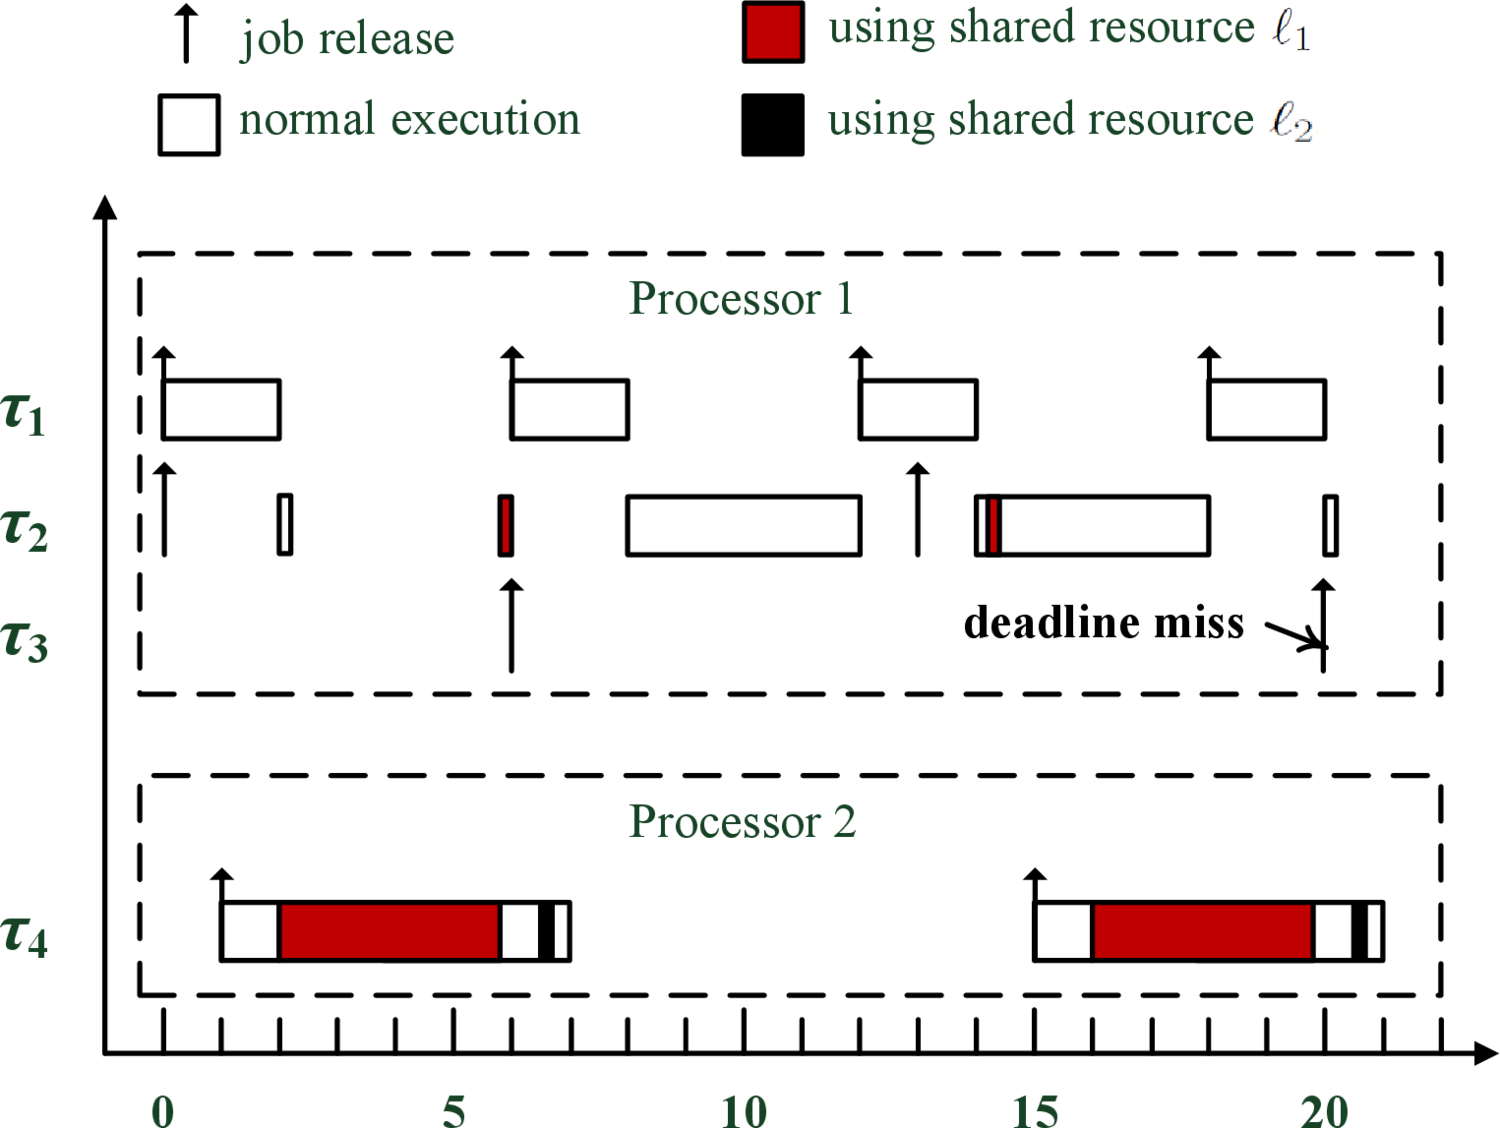
\includegraphics[width=12cm]{Counterexample}
\caption{An example schedule in which $\tau_3$ misses a deadline. 
}
\label{fig:counterexample_protocol}
\end{center}
\end{figure}


\begin{table}
\centering
    \begin{tabular}{|c|c|c|c|c|c|} 
 \hline
        $\tau_k$ & $C_k$ & $T_k$ ($= D_k$) & $s_k$ & $C_{k,1}^{\prime}$ & $C_{k,2}^{\prime}$\\
        \hline
        $\tau_1$ & 2             & 6  & 0 & 0 & 0\\ 
        $\tau_2$ & $4+2\epsilon$ & 13 & 1 & $\epsilon$ & 0\\
        $\tau_3$ & $\epsilon$    & 14 & 1 & 0 & $\epsilon$\\
        $\tau_4$ & 6             & 14 & 2 & $4-\epsilon$ & $\epsilon$\\ 
        \hline
    \end{tabular}
    \caption{Task parameters}
    \label{table:parameters}
\end{table}

Consider four implicit deadline sporadic tasks ${\tau_1, \tau_2, \tau_3, \tau_4}$ (with parameters listed in Table \ref{table:parameters}), ordered by decreasing order of priority, that are scheduled on two processors using P-FP scheduling. $\tau_1$, $\tau_2$ and $\tau_3$ are assigned to processor 1, while $T_4$ is assigned to processor 2. Jobs of $\tau_2$ each once use a global shared resource $\res_1$  ($s_2 = 1$) for a duration of at most $\varepsilon < 1$ ($C_{2,1}^{\prime} = \varepsilon$), where $\varepsilon$ an arbitrarily small, positive number. While jobs of $\tau_3$ each once use a global shared resource $\res_2$  ($s_3 = 1$) for a duration of at most $C_{3,1}^{\prime} = \varepsilon$. Jobs of $\tau_4$ each once use $\res_1$ for a duration of at most $C_{4,1}^{\prime} = 4-\varepsilon$, and each once use $\res_2$ for a duration of at most $C_{4,2}^{\prime} = \varepsilon$. 

Consider the response-time of $\tau_3$. Since $\tau_3$ is the lowest-priority task on its processor, it does not incur any local blocking (\ie,$s_3 \sum_{\tau_l \in \fun{lp}(3) \cap P(\tau_3)} \max_{1 \leq j < s_l} C_{l,j}^{\prime} = 0$). While each time $\tau_3$ requests $\res_2$, it may be delayed by $\tau_4$ for at most $\epsilon$. Thus, the maximum remote blocking of $\tau_3$ is bounded by $B_3^r = \epsilon$. With regard to the remote blocking incurred by each higher-priority task, we have $B_1^r = 0$ because $\tau_1$ does not request any global resource. Further, each time when a job of $T_2$ requests $\res_1$, it may be delayed for a duration of at most $4-\varepsilon$, thus $B_2^r = 4-\varepsilon$.\footnote{In general, the upper bound on blocking of course depends on the specific locking protocol in use, but in this example, by construction, the stated bound holds under any reasonable locking protocol. Recent surveys of multiprocessor semaphore protocols may be found in \cite{bbb-2013,yang-2015}.} Therefore, according to Eq. \ref{eqn:wcrt}, we have
\begin{align*}
& R_3^0 = \varepsilon + \varepsilon = 2\varepsilon, \\
& R_3^1 = 2\varepsilon + 0 + \left \lceil \frac{2\varepsilon + 0}{6} \right \rceil \cdot 2 + \left \lceil \frac{2\varepsilon + 4 - \varepsilon}{13} \right \rceil \cdot (4+2\varepsilon) =  6+4\varepsilon, \\
& R_3^2 = 2\varepsilon + 0 + \left \lceil \frac{6+4\varepsilon + 0}{6} \right \rceil \cdot 2 + \left \lceil \frac{6+4\varepsilon + 4-\varepsilon}{13} \right \rceil \cdot (4+2\varepsilon) = 8+4\varepsilon, \\
& R_3^3 = 2\varepsilon + 0 + \left \lceil \frac{8+4\varepsilon + 0}{6} \right \rceil \cdot 2 + \left \lceil \frac{8+4\varepsilon + 4-\varepsilon}{13} \right \rceil \cdot (4+2\varepsilon) = 8+4\varepsilon.
\end{align*}
 
As a result, $R_3 = 8+4\varepsilon < 14 = D_3$, and $\tau_3$ is considered to be schedulable according to the analysis in \cite{lakshmanan-2009}. However, there exists a schedule, shown in Fig. \ref{fig:counterexample_protocol}, where $\tau_3$  actually misses a deadline at time~20, which implies that Eq. \ref{eqn:wcrt} does not always yield a sound response-time bound. 

\subsection{Incorrect Time Request Analysis With Global Resource Sharing}

A related problem affects an \emph{interface-based analysis}  proposed by \cite{NBN:11}. Targeting \emph{open} real-time systems with globally shared resources (\ie, systems where the final task set composition is not known at analysis time, but tasks may share global resources nonetheless), the goal of the interface-based analysis is to extract a concise abstraction of the constraints that need to be maintained in order  to guarantee the schedulability of all tasks. In particular, the analysis seeks to determine the \emph{maximum tolerable blocking time}, denoted $\fun{mtbt}_k$, that a task $\tau_k$ can tolerate without missing its deadline. 

Recall from classic uniprocessor time-demand analysis \cite{lehoczky-1989} that, \emph{in the absence of jitter or self-suspensions}, a task $\tau_k$ is considered schedulable if
\begin{equation}
\label{eqn:rbf-1}
\exists t \in (0,D_k]: \fun{rbf_{FP}}(k,t) \leq t, 
\end{equation}
where $\fun{rbf_{FP}}(k,t)$ is the \emph{request bound function} of $\tau_k$, which is given by

\begin{equation}
\label{eqn:rbf-2}
\fun{rbf_{FP}} = C_k + B_k + \sum_{\tau_i \in \fun{hp}(k)} \left \lceil \frac{t}{T_i} \right \rceil \cdot C_i.
\end{equation}

Starting from Eq. \ref{eqn:rbf-1}, \cite{NBN:11} first  replaced $\fun{rbf_{FP}}(k,t)$ with its definition, and then substituted  $B_k$ with $\fun{mtbt}_k$. Solving for $\fun{mtbt}_k$ yields:
\begin{equation}
\label{eqn:bloc-tolerate}
\fun{mtbt}_k = \max_{0<t \leq D_k} \left( t - ( C_k + \sum_{\tau_i \in \fun{hp}(k)} \left \lceil \frac{t}{T_i} \right \rceil \cdot C_i ) \right).
\end{equation}

However, based on the example in secition \ref{sec:counterexample}, we can immediately infer that Eq. \ref{eqn:rbf-1} and Eq. \ref{eqn:rbf-2}, which ignore the effects of deferred execution due to remote blocking, are unsound in the presence of global locks. Consider $\tau_3$ in the previous example (with parameters listed in Table \ref{table:parameters}). According to Eq. \ref{eqn:bloc-tolerate}, we have $\fun{mtbt}_3 \geq 12 - (\epsilon + \lceil 12 / 6 \rceil \cdot 2 + \lceil 12 / 13 \rceil \cdot (4+2\epsilon)) = 4-3\epsilon$ (for $t=12$), which implies that $\tau_3$ can tolerate a maximum blocking time of at least $4-3\epsilon$ without missing its deadline. However, this is not true since $\tau_3$ can miss its deadline even without incurring any blocking, as shown in Fig. \ref{fig:counterexample_protocol}. 

\subsection{A Safe Response Time Bound}
\label{sec:safe_bound}

In Eq. \ref{eqn:wcrt}, the remote blocking of each higher-priority task (\ie, $B_i^r$) is counted in a similar way as release jitter. However, it is not sufficient to count the duration of remote blocking as release jitter, as already explained in section XXX. A straightforward fix is thus to replace $B_i^r$, in the ceiling function (\ie, the second term in Eq. \ref{eqn:wcrt}), with a larger value such as $D_i$ (as proved/discussed in section XXX) or $R_i - C_i$ (as proved / discussed in section XXX). Similarly, replacing $\sum_{\tau_i \in \fun{hp}(k)} \lceil t / T_i \rceil \cdot C_i$ in Eq. \ref{eqn:rbf-2} and Eq. \ref{eqn:bloc-tolerate} with $\sum_{\tau_i \in \fun{hp}(k)} \lceil (t+D_i) / T_i \rceil \cdot C_i$ or $\sum_{\tau_i \in \fun{hp}(k)} \lceil (t+R_i-C_i) / T_i \rceil \cdot C_i$ can fix the over-optimistic problem in \cite{NBN:11}.

Further, since \cite{zeng-2011,bbb-2013,yang-2013,kim-2014,han-2014,carminati-2014,yang-2014} reviewed in section \ref{sec:papers} merely reused the over-optimistic analysis approach introduced in \cite{lakshmanan-2009}, the stated fix may be used to correct the response-time tests in these papers without additional changes.